\documentclass[12pt]{article}

\usepackage[margin=0.5in]{geometry}
\usepackage{graphicx}
\usepackage{float}
\usepackage{titlesec}
\usepackage{parskip}
\usepackage{hyperref}

\titleformat{\section}{\large\bfseries}{\thesection.}{0.5em}{}
\titleformat{\subsection}{\normalsize\bfseries}{\thesubsection}{0.5em}{}

\title{\textbf{Prototype Overview: Automated Solar Panel Cleaning System}}
\author{Team 0104A}
\date{}

\begin{document}

\maketitle

\section{Introduction}

This document presents a comprehensive overview of the design, fabrication, integration, and verification of the Phase 3 Prototype System for the automated solar panel cleaning solution. The objective of this prototype was to validate the feasibility of a non-abrasive, film-based cleaning mechanism capable of removing dust while maintaining high light transmission and minimizing material consumption.

The final as-built prototype consists of a belt-driven transparent film system actuated by a stepper motor and controlled via a microcontroller with light-based activation. This document summarizes the system architecture, detailed design, key design decisions, integration challenges, and performance relative to the developed specifications, while referencing supporting artifacts across the Design Dossier.

\section{System Architecture}

\subsection{Mechanical Design}

The structural frame was constructed from machine plywood (approximately 25 cm $\times$ 20 cm), selected for rapid fabrication and ease of modification (see \href{}{04.2 Build}). Two parallel GT2 timing belts are routed along the frame and supported by front and rear idler pulleys mounted on wooden dowels.

A transparent polymer film spans the width of the system and is mechanically attached to the belts. The film travels across the acrylic panel surface, acting as a sacrificial cleaning interface. Unlike the conceptual design, the implemented system required the addition of a secondary film layer above the belts to ensure proper contact due to pulley height constraints.

Dust removal is achieved through a passive cleaning mechanism consisting of a microfiber cloth positioned along the return path of the film near the rear shaft. This location was selected to maximize cleaning effectiveness due to increased tension in the film during bending.

\subsection{Electrical Design}

The system is driven by a single NEMA 17 stepper motor connected to a shared wooden dowel shaft via a 3D-printed coupler. This configuration ensures synchronized motion across both belts (see \href{https://docs.google.com/document/d/1SjXE1apFuHjjCuuLbA2FhoU220ktpOhYzkgukCrVGak/edit?tab=t.0#heading=h.u59ujjk9x2b2}{03-ConceptualDesign: Pros and Cons Converging}).

Motor control is achieved using an A4988 stepper driver, which interfaces with the Raspberry Pi Pico W microcontroller. The electrical subsystem was designed to minimize component count while ensuring sufficient torque to overcome frictional resistance (see 04.3 Integration).

\subsection{Software Design}

The control system utilizes a photoresistor (LDR) to detect reductions in light intensity caused by dust accumulation. Upon detecting a threshold drop in light transmission, the Pico W triggers a single motor rotation cycle.

This represents a significant deviation from the original periodic actuation concept, introducing an event-driven control strategy that reduces unnecessary energy consumption and aligns with system objectives for low intervention (see \href{https://drive.google.com/drive/u/4/folders/1BAiKmYneszaR3hTWZbHwuF2bdrrcZR0l}{04.1 Prototype Feedback Notes and Resulting Iteration} and \href{https://docs.google.com/spreadsheets/d/1ZgWdYc8OaodtdYpCcwwQakVWo96tWj5T/edit?gid=1861155477#gid=1861155477}{04.4 VerificationProtocol+Results} ).

Figure 1 presents the system architecture of the as-built Prototype System, illustrating the interaction between the mechanical, electrical, and software subsystems.

\begin{figure}[H]
    \centering
    
    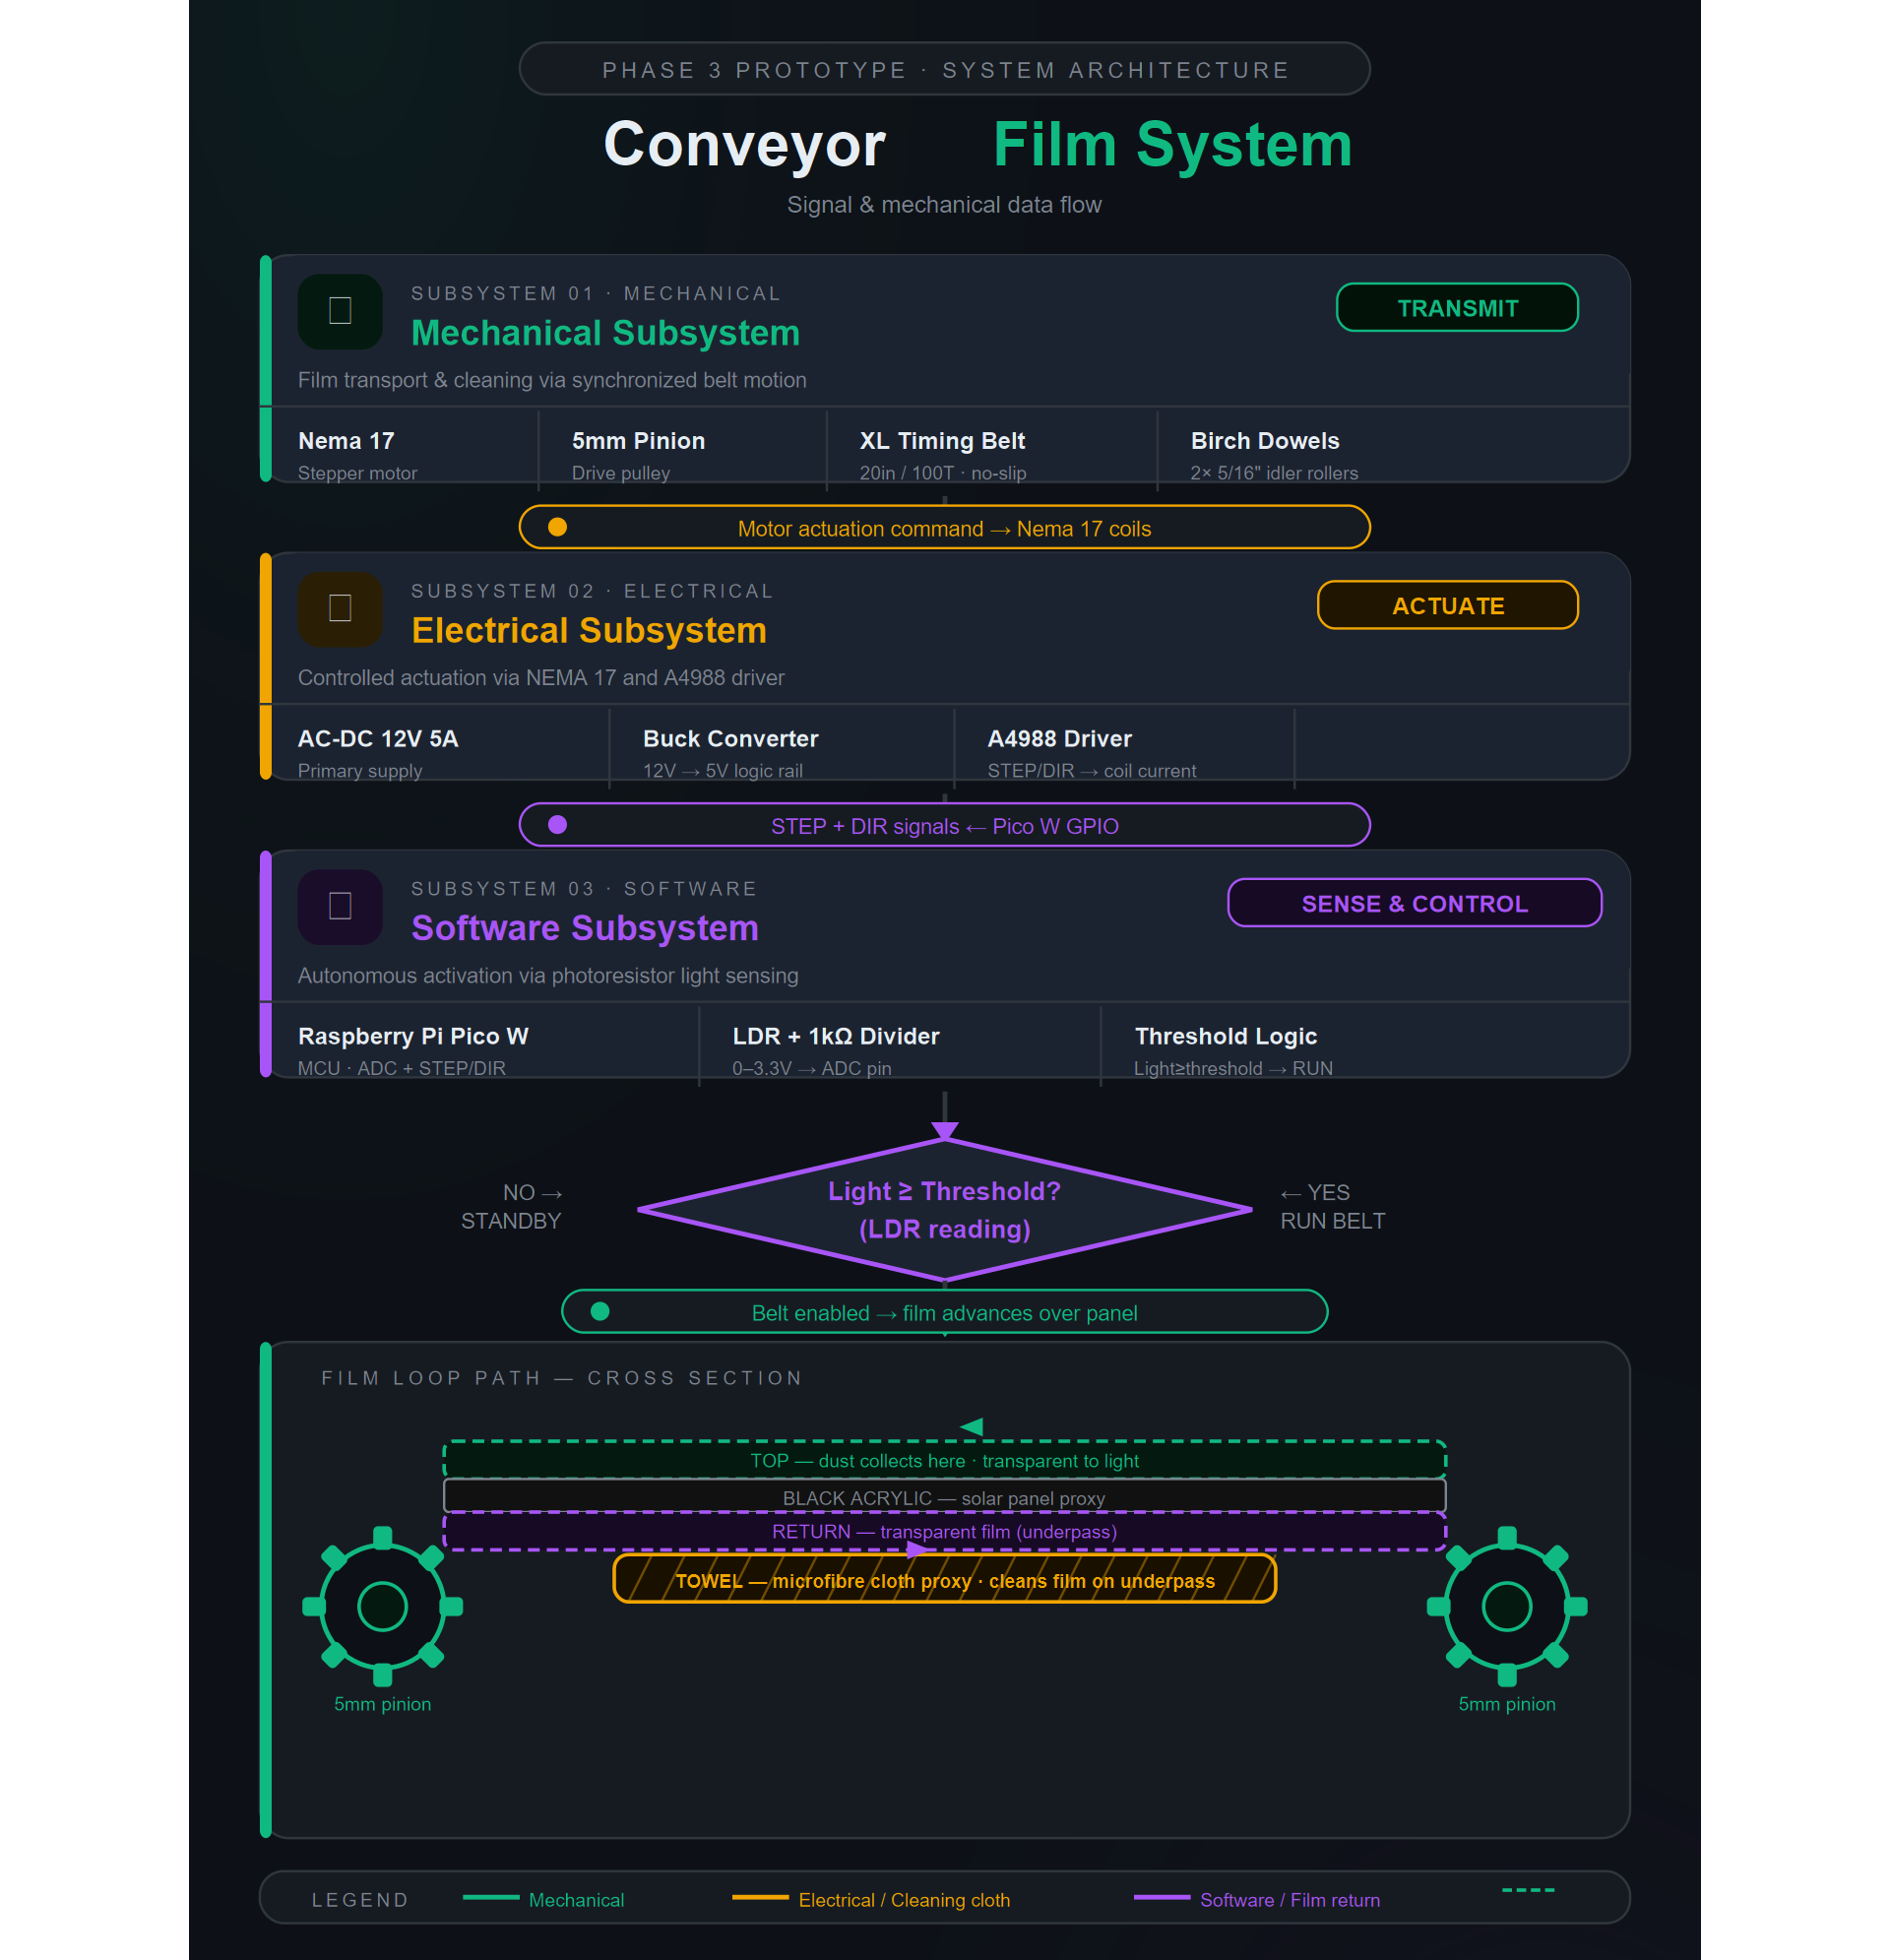
\includegraphics[width=0.8\linewidth]{assets/conveyor_flowchart.png}
    
    \caption{System architecture of the as-built prototype system.}
\end{figure}

The system integrates three primary subsystems:

\textbf{Mechanical Subsystem:} Responsible for film transport and cleaning action through synchronized belt motion.

\textbf{Electrical Subsystem:} Provides controlled actuation using a NEMA 17 stepper motor and A4988 driver.

\textbf{Software Subsystem:} Enables autonomous activation through a photoresistor-based light sensing mechanism.

 Here is a more detailed overview of the \href{https://docs.google.com/document/d/1Fe0dRtZV8c90UYq46zju22RK1K1eeR_mjBnPMjBk4DA/edit?tab=t.0}{04.1-System Architecture}

\section{As-Built Prototype System}

\begin{figure}[H]
    \centering
    \fbox{\parbox{0.7\textwidth}{
    \centering
    \textbf{PLACEHOLDER: As-Built Prototype Photo}

    \vspace{0.5em}
    \textit{Insert real image showing full assembly: frame, belts, film, motor}
    }}
    \caption{As-built prototype system.}
\end{figure}

The final prototype differs from the initial design concept in several critical ways, reflecting practical constraints and iterative refinement during Phase 3.

\section{Design Process and Iteration}

The design process followed a structured iterative workflow consisting of divergence, convergence, fabrication, and integration stages.

Initial concept generation and evaluation were conducted using brainstorming, SCAMPER, and Pugh analysis methods (see \href{https://drive.google.com/drive/u/4/folders/1H7HwvAO-qYqSBoSMpMYzfeY-mcBnA41G}{03-Conceptual Design}). These were followed by a trade-off analysis to converge on final subsystem decisions, including motor selection, film material, and attachment methods.

Fabrication (see 04.2 Build) involved rapid prototyping using MyFab resources, enabling quick iteration on frame geometry and shaft configurations. Integration (see 04.3 Integration) revealed several mechanical and alignment challenges, which required refinement of shaft interfaces, belt alignment, and friction reduction strategies.

This iterative process ensured that the final prototype reflects both design intent and practical constraints encountered during implementation.

\section{Key Design Decisions}

Several critical design decisions significantly influenced the performance and feasibility of the prototype:

\textbf{Single Motor Drive System:} A single NEMA 17 motor driving a shared shaft was selected over dual motors to eliminate synchronization issues and ensure uniform belt motion.

\textbf{Transparent Film Selection:} A MyFab-sourced plastic sheet was chosen for its durability and flexibility, balancing optical clarity with mechanical robustness.

\textbf{Stitched Film Attachment:} Stitching was selected over adhesive methods for improved reliability during repeated cycles.

\textbf{Plywood Frame Construction:} Laser-cut plywood enabled rapid iteration and sufficient structural integrity for the prototype scale.

\textbf{Photoresistor-Based Control:} Transitioning from periodic activation to light-triggered control improved energy efficiency and reduced unnecessary operation.

These decisions are supported by trade-off analysis and documented in 04.1 PrototypeDesign.

\section{Integration Challenges and Debugging}

During integration, several significant challenges were encountered:

\textbf{Pulley Height Mismatch:} The belt sat below the pulley edges, preventing proper film contact. This was resolved by layering additional material to raise the belt surface.

\textbf{High Friction in Shaft Supports:} Wood-on-wood contact created excessive resistance. This was mitigated by introducing a metal shaft coupler, reducing friction and improving rotational smoothness.

\textbf{Dowel Sizing Constraints:} Available dowel sizes did not match pulley interfaces, leading to alignment issues. The final solution utilized smaller dowels secured with screws to ensure proper alignment and consistent rotation.

These challenges and their resolutions are documented in detail in 04.3 Integration.

\section{Performance Relative to Specifications}

The prototype system was evaluated against key specifications (see \href{https://docs.google.com/spreadsheets/d/19Sxo5atl2CzB1H0pCT4QkIaBSSTG0vjS/edit?gid=1424656124#gid=1424656124}{04-Specification}):

\textbf{Dust Removal (OM-1.1):} The microfiber cleaning mechanism demonstrated effective removal of surface dust following a single rotation cycle.

\textbf{Light Transmission (OM-1.2, OM-1.3):} The transparent film maintained high light transmission, with observable improvement after cleaning.

\textbf{Material Usage (OM-2.1):} The system operates without water or disposable components, meeting sustainability objectives.

\textbf{Mechanical Safety (OM-2.6):} The film maintained clearance above the panel, preventing surface damage.

\textbf{Electrical Performance (OE-1.1, OE-1.4):} The motor consistently achieved a complete rotation without stalling, with controlled cycle duration.

\textbf{Software Control (OS-1.1, OS-1.5):} The system successfully triggered autonomous cleaning cycles based on light conditions with no user intervention.

Overall, the prototype meets all primary functional requirements and demonstrates feasibility of the proposed design.

\section{Validation of Design Concept}

The prototype provides strong validation of the core design concept by demonstrating that:

\begin{itemize}
    \item A moving transparent film can effectively transport dust away from a surface.
    \item Passive microfiber cleaning can prevent re-deposition.
    \item Non-contact cleaning reduces risk of panel damage.
    \item Autonomous activation is feasible using simple sensing mechanisms.
\end{itemize}

However, several considerations remain for future development:

\begin{itemize}
    \item Long-term durability of the film under environmental exposure
    \item Optimization of film tension and cleaning pressure
    \item Scalability to full-size solar panels
\end{itemize}

\section{Conclusion}

The Phase 3 prototype successfully demonstrates the feasibility of an automated, non-abrasive solar panel cleaning system. Through iterative design, integration, and testing, the system validates key functional requirements while highlighting areas for future refinement. The results support the viability of the proposed design concept for further development and scaling.

\end{document}